
Sudoku is a constraint satisfaction puzzle where each row, column and block must contain each symbol exactly once. This project focuses on small binary Sudoku variants that are able to run on a quantum computer: a $2\times 2$ Sudoku (4 cells) and a $4\times 4$ Sudoku (16 cells). 
% To make both simulations and hardware run for the $4\times 4$ 

% To make a hardware run for the $4\times 4$ case feasible, partially filled puzzles are used with only about 6 empty cells. This reduces the number of unknowns and therefore the number of data qubits and the necessary circuit depth, which helps produce meaningful results on current IBM devices.

\paragraph{Classical approach:}
For baseline comparisons standard classical methods are used. The $2\times 2$ case is solved by exhaustive checking of all assignments. For the $4\times 4$ instances a backtracking solver is used with simple pruning (row/column/block constraints). These classical solvers exploit constraint structure and are extremely fast on classical computers for the instance sizes considered, typically finishing in milliseconds or less.

\paragraph{Quantum formulation:}
Each unknown cell is encoded as a qubit (one qubit per binary cell value) and build a reversible oracle \(U_f\) that marks assignments satisfying all row, column and block constraints. Ancilla qubits implement temporary parity and uniqueness checks using CNOTs and multi-controlled gates, making the check reversible. The algorithm starts in an equal superposition over the $N=2^{\#\text{possible values}}$ candidate assignments, and then repeats Grover iterations (oracle + diffusion). The approximate number of Grover iterations is
\[
k \approx \frac{\pi}{4}\sqrt{\frac{N}{M}},
\]
where \(M\) denotes the number of satisfying assignments. For a partially filled \(4 \times 4\) puzzle with approximately six unknown variables, and using two qubits per unknown to encode each possible value, a total of 12 qubits is required. This results in a search space size of \(N \approx 2^{12} = 4096\). Assuming a single valid solution (\(M = 1\)), the expected number of Grover iterations is on the order of 50.


\vspace{1em}
\noindent A key practical point is that the main limiter for running these circuits on cloud quantum hardware is gate depth, not raw qubit count. Although providers such as IBM have devices with many physical qubits, deep circuits with many sequential two- (or more) qubit gates quickly accumulate errors and cause decoherence. To see more about the theoretical capabilities of a Quantum Computer, the sudoku algorithm was also run using the AerSimulator of Qiskit. However, classical simulation faces its own severe scalability constraints due to the exponential growth of quantum state space. Simulating a completely empty $4\times 4$ Sudoku requires 32 logical qubits just to encode the variables. A statevector simulation of this size requires a minimum of 64 GB of RAM for the amplitudes alone, excluding overhead for ancilla qubits and gate operations. Furthermore, the search space of \(2^{32}\) states would require over \textbf{50,000} Grover iterations, making full simulation unfeasible.

\vspace{1em}
\noindent Therefore a partially filled $4\times 4$ instance was chosen to keep the overall circuit depth and the number of multi-qubit gates low enough to obtain useful results. Also, optimizations in terms of the ancillae used had to be done. To minimize qubit overhead, the oracle implements a batch processing strategy where constraints are evaluated in blocks of four, instead of assigning a unique ancilla to every constraint, which would require much more qubits. For each block, constraints are computed in temporary ancillae, and their results are added to a results register using a multi-controlled X gate. The block ancillae are then uncomputed to prepare them for the next batch.

\vspace{1em}
\noindent
The total number of constraints proved to also be a critical balancing factor in the circuit design. Each additional constraint increases the computational cost in two ways: it requires more logical gates to verify (increasing the oracle depth) and often necessitates additional ancilla qubits or reuse cycles. Theoretically, a set of all the needed constraints is needed to ensure the puzzle has a unique solution (M=1), which allows Grover’s algorithm to amplify the correct state probability to nearly 100\%, if the number of iterations is sufficient. Therefore, a minimal set of 28 constraints was selected, to minimize qubit overhead, and careful classical pre-processing was done to get a unique solution without adding redundant checks that would unnecessarily inflate the circuit depth.

\vspace{1em}
\noindent Typical resource estimates for the partially filled $4\times 4$ run on quantum hardware are:
\begin{itemize}
  \item Data qubits: 12 (two per unknown cell as to encode 4 values).
  \item Ancilla qubits: $\sim 13$--14 
  \item Total qubits after overhead: $\sim 25$--26. (depends on the placement and number of empty cells)
  \item Planned Grover iterations: $k\approx$ 50.
\end{itemize}

% \paragraph{Results.}
% We ran the $2\times 2$ Sudoku on an IBM device as a proof of concept and executed the partially filled $4\times 4$ instance on hardware as described above. For each circuit (with a fixed number of Grover iterations) we collected many shots, in our case 4096, to estimate frequency distributions of measured bitstrings. The runs were also executed in a noiseless Qiskit simulator to provide the ideal reference distribution.

% \vspace{1em}
% \noindent The hardware results show the expected Grover amplification pattern: the correct solutions appear more frequently near the predicted number of iterations, but with a lower success probability than the simulator due to noise and decoherence of the quantum hardware the code is run on. Because Grover is probabilistic, we report probabilities by dividing the measured outcomes by the shot count. The following histogram summarizes the hardware measurements for both the $2\times 2$ and the partially filled $4\times 4$ runs.

% \vspace{1em}
% \noindent We also executed the Grover search for the partially filled 4×4 Sudoku (6 unknowns) on both a noiseless simulator and the ibm\_torino quantum processor. The logical circuit required approximately 28,000 quantum gates and was set to run for 50 iterations, the theoretically optimal number calculated for this problem size.

% \begin{figure}[H]
%     \centering
%     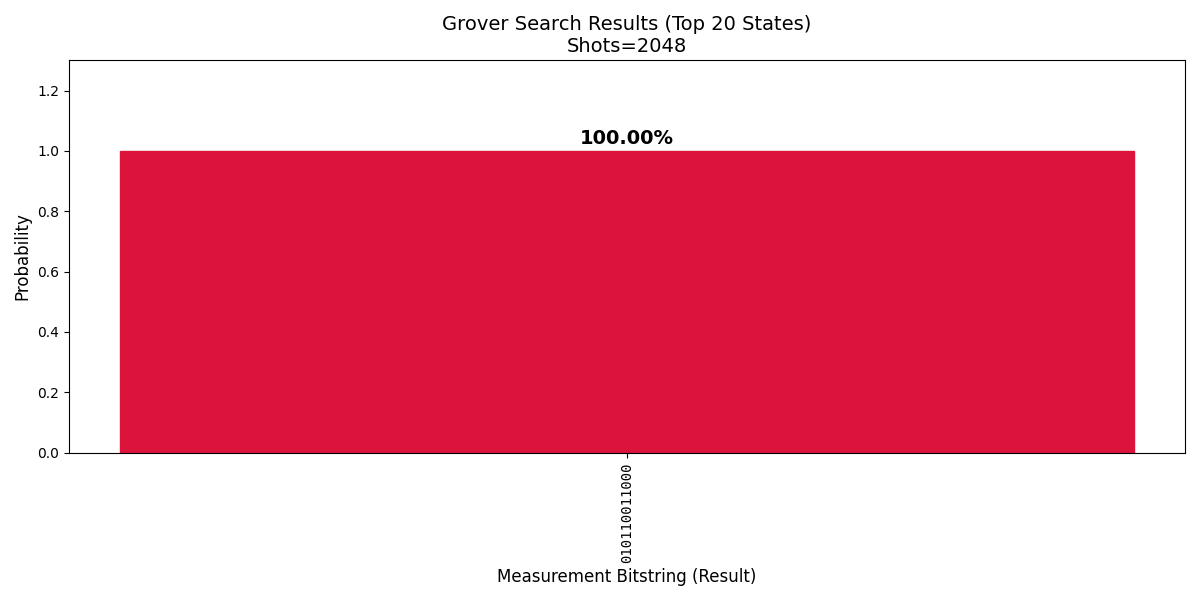
\includegraphics[width=1\linewidth]{Simulator_2.png}
%     \caption{Simulation with 50 iterations}
%     \label{fig:placeholder}
% \end{figure}

% \noindent The algorithm was run on the Qiskit Aer Statevector simulator. Figure 1 demonstrates the algorithm's logical correctness: the probability of measuring the correct solution state (\texttt{010110011000}) reached 100\%, confirming that the Oracle and Diffuser were constructed correctly and capable of amplifying the solution in a noise-free environment. This can be seen also in Figure X, where for 45 iterations the probability goes down to 97.61\%, and for 25 to 50\%.

% \begin{figure}[H]
%     \centering
%     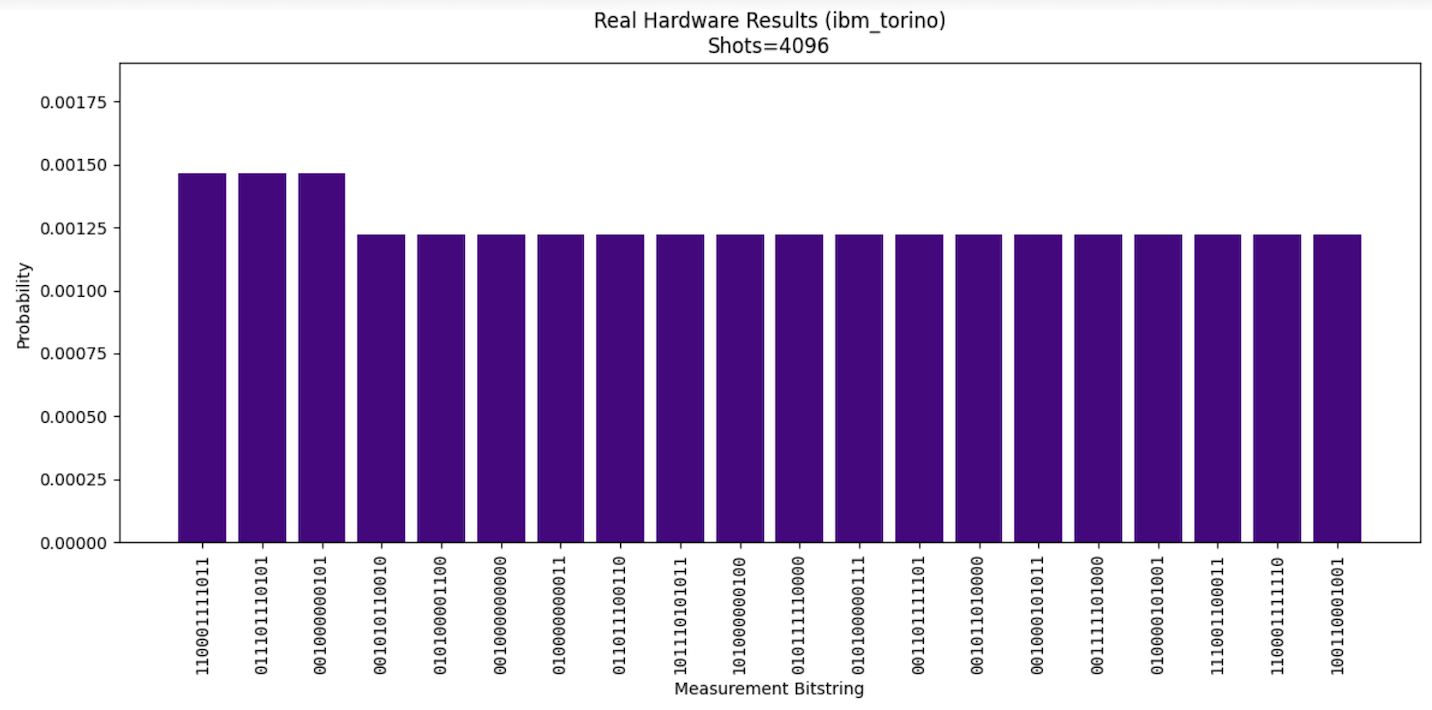
\includegraphics[width=1\linewidth]{Screenshot 2026-01-23 at 21.42.32.png}
%     \caption{Experimental results on \texttt{ibm\_torino} (4096 shots). The distribution is flat, indicating that the quantum state decohered into random noise before the computation could complete.}
%     \label{fig:placeholder}
% \end{figure}

% \noindent When the circuit was executed on the ibm\_torino backend (133 qubits), the results were drastically different. As shown in Figure 2, the probability distribution is indistinguishable from uniform random noise ($\sim$ 0.015\%). The amplification observed in the simulator was completely lost.
% \vspace{1em}
% \noindent To understand the discrepancies between the simulation and the hardware execution, we analyzed the circuit compilation and the probability of the algorithm to find the correct answer in both theoretical and real scenarios.

% \begin{figure}[H]
%     \centering
%     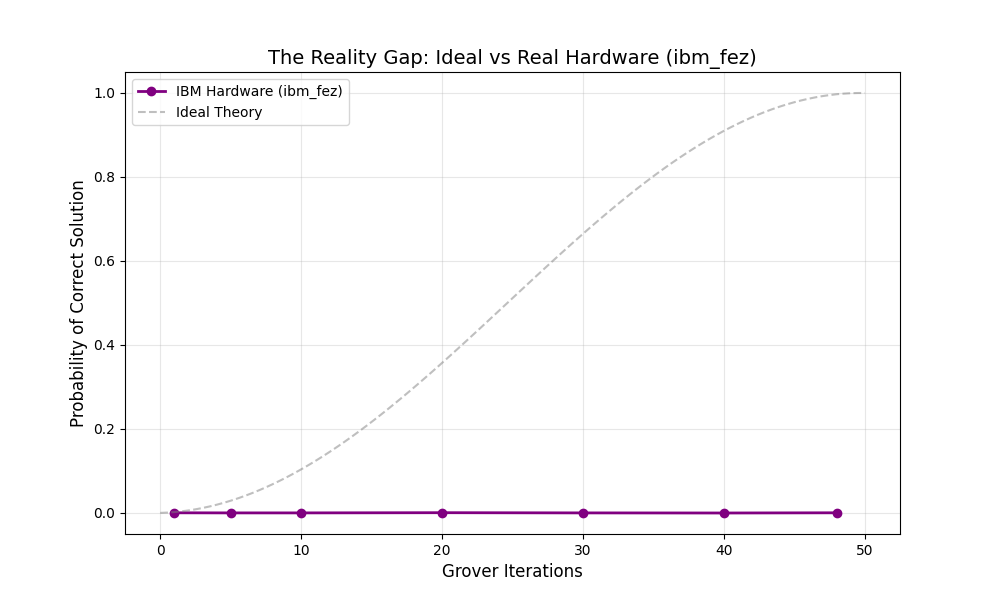
\includegraphics[width=1\linewidth]{ibm_death_curve.png}
%     \caption{The probability difference analysis. The ideal probability (grey) rises to 100\%, while the real hardware probability (purple) never deviates from zero, showing that noise dominates the signal instantly.}
%     \label{fig:placeholder}
% \end{figure}

% \noindent We performed a depth-sweep experiment, running the algorithm for $k={1,5,10,…,50}$ iterations on hardware. Figure 3 illustrates the gap between the simulation and the real capabilities of a current Quantum Computer. While theory predicts a smooth sinusoidal rise in probability (grey line), the hardware success rate (purple line) remains flat at zero even for shallow depths. This indicates that the circuit depth exceeded the qubit coherence time ($T1/T2$) almost immediately.

% \vspace{1em}
% \noindent The primary cause of this failure was identified in the transpilation phase of the process. The logical circuit contained $\sim$28,100 gates, and to map this to the physical hardware the insertion of SWAP gates was required to satisfy connectivity constraints. This caused a massive increase in the gate count to 785,780 and the circuit depth to 290,053. Given that current superconducting qubits can typically sustain only a few thousand gates before decoherence, a depth of 290,000 makes successful computation physically impossible for the now-available hardware.

% \paragraph{Summary.}
% Overall, the Sudoku experiments show both the strengths and limitations of Grover’s algorithm on current quantum hardware. For very small instances such as the $2\times 2$ Sudoku with some pre-filled values, Grover’s algorithm performs reliably and produces results close to the ideal theoretical prediction. This case serves as a good demonstration of running Grover's algorithm on real quantum hardware.

% \vspace{1em}
% \noindent For larger instances, such as the partially filled $4\times 4$ Sudoku, the quadratic speed-up offered by Grover’s algorithm is still present in theory, but its practical benefit is reduced by hardware noise and circuit depth. Even though sufficient qubits are available, error accumulation limits the number of Grover iterations that can be applied before the output becomes unreliable. On top of that, classical solvers can make use of this underlying structure of sudoku and perform way better than the theoretical runtime complexity. These results show that, for structured problems like Sudoku, classical solvers remain more efficient and practical in possibly all cases, while quantum approaches mainly serve as a proof-of-concept for studying scalability, noise effects, and future hardware improvements.